\chapter{Revisão de Literatura}
\label{cap:revisao}
Este Capítulo apresenta uma revisão de literatura essencial para a compreensão do trabalho. Dentre os temas abordados, estão definições e arquitetura das SDNs (Seção \ref{sec:sdn}). O funcionamento e principais componentes relacionados ao protocolo \textit{OpenFlow} na configuração dos dispositivos (Seção \ref{sec:openflow}). A arquitetura do controlador \textit{floodlight} e o e funcionamento de aplicações suportadas (Seção \ref{sec:floodlight}). Por fim as considerações em relação aos conceitos apresentados para a compreensão do próximo capítulo é apresentado em (Seção \ref{sec:consider})

%////////////////////////////////////////////////////////////////////////////////////
\section{Redes Definidas por Software}
\label{sec:sdn} %\pagebreak

Em redes tradicionais, comutadores normalmente possuem sistemas fechados de gerenciamento e configuração disponibilizados pelos fornecedores dos dispositivos, dificultando a evolução de novos protocolos e tecnologias para gerenciamento de infraestruturas de comunicação. Essa característica, reduziu a flexibilidade da evolução arquitetural e dos protocolos~\cite{handley2006internet}, principalmente devido a camada de controle e camada de dados embutidas em cada dispositivo de encaminhamento como mostrado na Figura~\ref{fig:control_data_plane}~(a). 

SDN é um paradigma emergente que possibilita mudanças para as limitações apresentadas em redes tradicionais. Em SDN, a separação do plano de controle e do plano de dados permite que os comutadores da rede se tornem simples dispositivos de encaminhamento, enquanto o controle gerencial da rede é centralizado em um controlador lógico chamado \emph{Network  Operation  System} (NOS) ~\cite{kreutz2015}, facilitando a utilização de novas aplicações e protocolos ~\cite{nunes-2014}. 

\begin{figure}[!htb]
	\caption{\label{fig:control_data_plane}Principal diferença entre ~\textit{a)} redes tradicionais e \textit{b)} SDN}
	\begin{center}
	    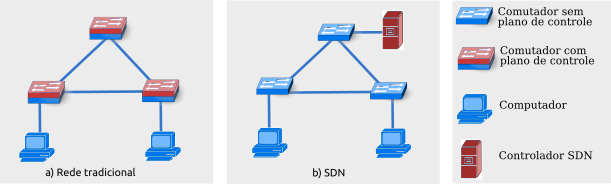
\includegraphics[scale=0.9]{imagens/diferenca.png}
	\end{center}
	\fonte{Elaborada pelo autor (2021), com base em \cite{nunes-2014}}
\end{figure}

A Figura ~\ref{fig:control_data_plane} ilustra duas infraestruturas de rede.
A primeira, \textit{(a)} corresponde a uma rede tradicional, ou seja, a camada de controle está embutida nos comutadores, de modo a realizar o roteamento de pacotes utilizando uma visão local (parcial) da rede. A segunda \textit{(b)}, ilustra uma infraestrutura SDN, seu plano de controle é separado em um ou mais controladores lógicos que utilizam a visão global da rede para efetuar o encaminhamento dos fluxos.

A abstração da camada de controle dos dispositivos em SDN permite que os comutadores atuem apenas como dispositivos de encaminhamento, baseado no conjunto de regras especificadas pelo controlador, conforme a política implementada. Um SDN pode ser apresentado como uma arquitetura de alto nível dividida em três principais planos funcionais, como ilustrado na Figura~\ref{fig:arquitetura_sdn}~(a), assim elencados: \textit{(i)} Plano de Dados,  envolve toda a infraestrutura da rede sendo composta por dispositivos de encaminhamento físicos ou virtuais, computadores e demais dispositivos terminais. 
\textit{(ii)} Plano de controle, responsável por consolidar funcionalidades através de Interfaces de Programação de Aplicações (APIs) que supervisionam o comportamento de encaminhamento dos comutadores. 
\textit{(iii)} Plano de gerenciamento, também conhecido como plano de aplicação, consiste em programas que fazem o uso das informações fornecidas pelo NOS para efetuar o gerenciamento da SDN~\cite{jarraya-2014}. 


\begin{figure}[!htb]
	\caption{\label{fig:arquitetura_sdn} Representação de um SDN em a) planos, b) camadas.}
	\begin{center}
	    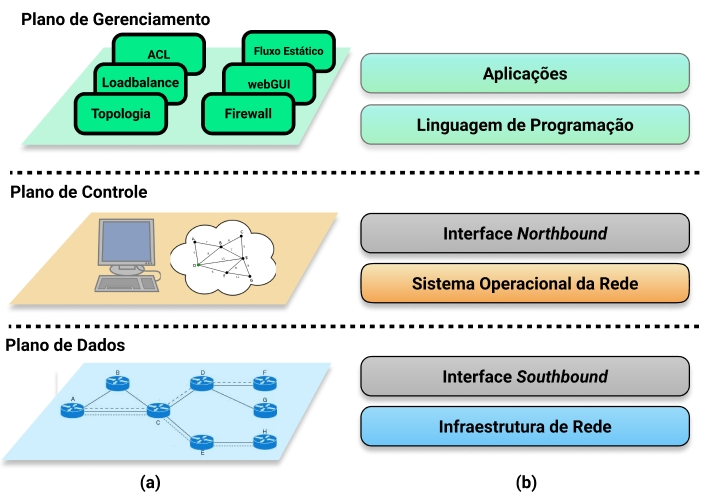
\includegraphics[scale=0.60]{imagens/planos_camadas.jpg}
	\end{center}
	\fonte{Elaborada pelo autor (2021), com base em \cite{kreutz2015}}
\end{figure}

A Figura ~\ref{fig:arquitetura_sdn} é uma representação simplificada das camadas que constitui um SDN. Políticas de controle de fluxos podem ser implementadas como uma aplicação do plano de gerenciamento ou ainda como um serviço estendendo funcionalidades e módulos no próprio controlador. Na primeira existe a vantagem de se poder criar aplicações portáveis que podem ser utilizadas em diversos controladores. Já a segunda opção da mais agilidade por ser executada diretamente no controlador.

%||||||||||||||||||||||||||||||||||||||||||||||||||||||||||||||||||||||||||||||||||||||||||||||||
\subsection{Fluxos de Dados}

Um fluxo é uma sequência de pacotes que correspondem a uma determinada comunicação entre dispositivos finais. Por exemplo, pode-se considerar que \textit{streaming} de vídeo realizado de um computador A para um computador B é um fluxo de dados. Já um caminho de fluxo corresponde a um sub conjunto de dispositivos SDN que possuem  regras em suas tabelas de modo que possam encaminhar os pacotes do fluxo de origem até o destino. 
No exemplo da Figura ~\ref{fig:reativo} um caminho de fluxo entre A e B é formado pelos comutadores 1 e 2 ligados de forma linear.
O caminho de fluxo é calculado pelo controlador SDN e pode ser realizado de maneira proativa ou reativa, conforme a abordagem selecionada pelo controlador para satisfazer os requisitos do fluxo como \emph{Quality of Service} (QoS), diminuição de latência~\cite{paulo:2016} ou melhor utilização da rede.
\begin{figure}[!htb]
	\caption{\label{fig:reativo}Diagrama de sequência, funcionamento da abordagem reativa.}
	\begin{center}
	    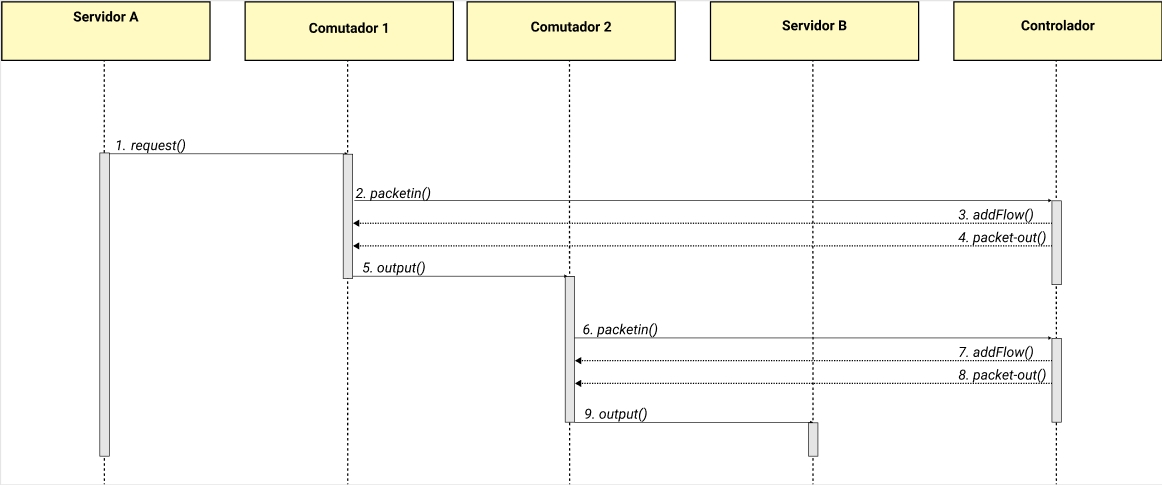
\includegraphics[scale=0.45]{imagens/Reativo.jpg}
	\end{center}
	\fonte{Elaborada pelo autor (2021).}
\end{figure}
A Figura~\ref{fig:reativo}, ilustra a ordem do processo de configuração dos dispositivos de rede utilizando a abordagem reativa. Neste cenário o servidor A envia um \emph{Address Resolution Protocol} (ARP) para fechar uma conexão com o servidor B. Ao chegar no primeiro comutador, este não possui nenhuma regra para tratar o pacote gerando assim o primeiro \textit{packet-in}, enviado ao controlador via canal seguro. O controlador verifica os campos do \textit{packet-in} e analisa junto a topologia global da rede gerando regras de fluxos, essas regras contém as ações de encaminhamento adicionado pelo comando \textit{addFlow}, criando em seguida um \textit{packet-out} devolvendo o pacote ao comutador. Quando o pacote chega ao próximo comutador este gera outro \textit{packet-in}, novamente o controlador adiciona as regras e em seguida devolve o pacote por um \textit{packet-out}. O mesmo processo se repete a cada salto até que todos os comutadores do caminho sejam configurados. 

Os demais pacotes que fazem parte do fluxo não geram \textit{packet-in} devido às regras inseridas durante o evento \textit{addFlow}. Este caminho permanece nos comutadores até que o \textit{time-out} vinculado a regra ocorra, ou ainda, caso o controlador remova a regra por motivos específicos. Os pacotes inseridos pelo \textit{addFlow} são similares aos do \textit{packet-out}, porém o primeiro contém instruções em seu conjunto de ações que servem para inserir, remover e atualizar as regras, já o segundo apenas ações de encaminhamento.
\begin{figure}[!htb]
	\caption{\label{fig:proativo}Diagrama de sequência, funcionamento da abordagem proativa.}
	\begin{center}
	    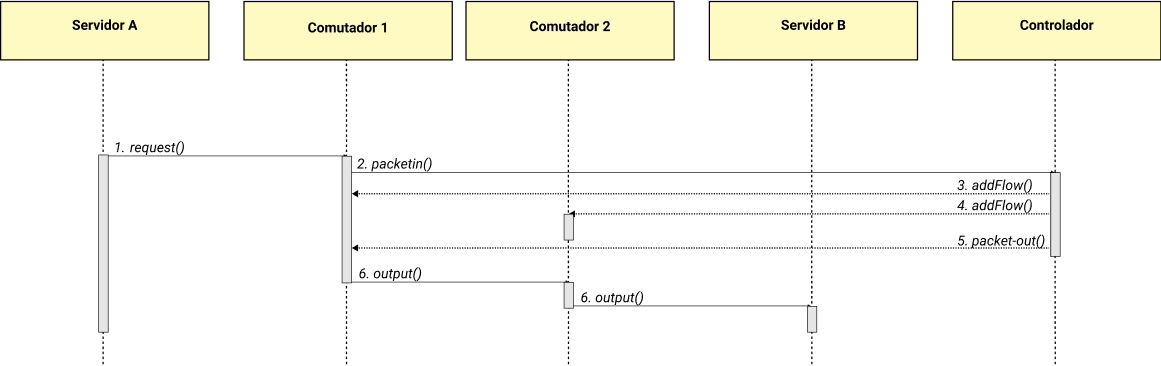
\includegraphics[scale=0.45]{imagens/Proativo.jpg}
	\end{center}
	\fonte{Elaborada pelo autor (2021).}
\end{figure}
%\todo{Alterar Servidor A para Servidor B}

Na abordagem proativa ilustrada pela Figura ~\ref{fig:proativo}, ao receber o primeiro \textit{packet-in} o controlador utilizara informações globais da rede para encontrar a lista de todos os dispositivos que compõem o caminho de A para B, conforme a política de encaminhamento implementada (\emph{e.g.,} Menor quantidade de saltos, menor tráfego, entre outros). Ao obter essa lista o controlador inicia o processo de configuração dos dispositivos, enviando instruções com configuração específica para cada comutador que compõe o caminho do fluxo. Com os dispositivos configurados, os próximos pacotes do fluxo seguem segundo as regras existentes nas tabelas de fluxos, assim cada novo fluxo gera apenas um \textit{packet-in}.


%||||||||||||||||||||||||||||||||||||||||||||||||||||||||||||||||||||||||||||||||||||||||||||||||
%\item Aplicação: \\
\subsection{Plano de Gerenciamento}

O plano de gerenciamento, ou plano de aplicações, interage com o controlador através da Interface de Programação de Aplicações (API) \textit{northbound}, para manipular serviços oferecidos pela rede. 
Nesta camada, se destacam duas linhas de pesquisas relacionadas com o objetivo do presente trabalho: \textit{(i)} aplicações SDN para gerenciar funcionalidades específicas da rede e \textit{(ii)} aplicações SDN para gerenciar ambientes específicos. O primeiro interage com o controlador para gerenciar necessidades particulares da rede categorizadas em domínios de segurança, QoS, engenharia de tráfego e balanceamento de carga. No segundo caso, as aplicações SDN focam em ambientes específicos tais como computação em nuvem, rede móvel, virtualização de rede e \emph{Network Functions Virtualization} (NFV) ~\cite{jarraya-2014}.

Uma SDN facilita o desenvolvimento de novas aplicações destinadas a segurança tal como \emph{OpenFlow Random Host Mutation} (OFRHM), que possuem técnicas que escondem componentes da rede de \textit{scanners} externos e internos que tentam descobrir alvos de possíveis ataques. Assim, endereços IPs virtuais são alocados dinamicamente  de tal forma que os hospedeiros evitem a exposição de seus IPs reais que podem ser usados para ataques~\cite{jafarian-2012}. Aplicações específicas para migração de MVs~\cite{ghorbani-2012} e realização de IP \textit{multicasting}~\cite{nakagawa2012} são facilitadas com SDN. Neste segundo, o protocolo permite que o registro seja efetuado dinamicamente permitindo que membros possam se juntar ou deixar o grupo de comunicação sem intervenção de gerenciamento da rede.

Ainda, aplicações de gerenciamento, como \textit{Access Control List}~(ACL), podem ser implementadas por um administrador.
Essas aplicações permitem a definição de políticas para tomada de decisão em novos fluxos adicionados para ser verificada em conjuntos de regras que permitam determinadas conexões, por exemplo (um servidor somente pode utilizar o protocolo HTTP se estiver utilizando \textit{proxy}). 
Complementarmente, aplicações para isolamento de redes também podem ser facilmente aplicadas, associando as portas que podem ser utilizadas por determinadas identificações de VLANs marcadas no cabeçalho do pacote, podendo também designar ações para que um pacote vindo de um determinado endereço físico ou IP seja marcado com uma identificação de VLAN. Em uma SDN aplicações de ACL contém regras que são consultadas durante um evento de \textit{packet-in}, permitindo ou impedindo a criação do fluxo. Já as aplicações de \textit{firewall} colocam essas regras nos comutadores permitindo o encaminhamento ou descartando o pacote através de uma ação \textit{drop}.
A maioria dos SDN utilizam endereçamento IP, no entanto, o \textit{OpenFlow} permite que aplicações façam o gerenciamento da rede de modo a não utilizar de endereço IP~\cite{mckeown2008}, tais como utilizar apenas a camada de rede \emph{Media Access Control} (MAC).


% Aplicações de gerenciamento como \textit{Network Management and Access Control} que permitem implantação de para tomada de decisão para novos fluxos adicionados para que seja verificada conjuntos de regras de como por exemplo (um host pode utilizar o protocolo HTTP apenas se estiver utilizando proxy, pu um telefone VoIP não pode se comunicar com laptops). Aplicações para isolamento de redes também podem ser facilmente aplicadas, associando as portas que podem ser utilizadas por determinadas identificações de VLANs marcadas no cabeçalho do pacote. Podendo também designar ações para que por exemplo um pacote vindo de um determinado endereço físico ou IP seja marcado com uma indentificação de VLAN. A maioria dos SDN utilizam endereçamento IP, mas no entanto o OpenFLow permite que aplicações façam o gerenciamento da rede de modo a não utilizar de endereço IP, utilizando apenas matches compatíveis com a camada de rede (endereço MAC)~\cite{mckeown2008}.





%||||||||||||||||||||||||||||||||||||||||||||||||||||||||||||||||||||||||||||||||||||||||||||||||
\subsection{Plano de Controle}

Denominado de NOS, é o responsável por fornecer as funcionalidades da rede. Ele contém o controlador que atua entre o plano de gerenciamento e o plano de dados~\cite{xie2015control}. Sendo assim, o controlador tem acesso às funcionalidades fornecidas pelo \textit{OpenFlow} da camada \textit{southbound}, e as fornecem como serviços para as aplicações por meio da \textit{interface northbound}.



\subsubsection{Interface Northbound} 

É uma camada de API que abstrai instruções de baixo nível da camada \textit{southbound} na configuração de entradas das tabelas de fluxos do plano de dados. A abstração pode ser feita através de linguagem de programação como \textit{Frenetic}~\cite{foster2011frenetic} e NetCore ~\cite{monsanto2012compiler}. APIs abertas ou padronizadas são importantes, pois fornecem portabilidade às aplicações podendo ser utilizadas em diferentes NOS. Alguns controladores como Floodlight ~\cite{floodlight2012}, NOX~\cite{nox2008} e OpenDaylight~\cite{opendaylight2014} possuem suas próprias \textit{northbound} APIs específicas para seus propósitos. Nessa camada é comum a utilização da API RESTfull que faz o uso do \emph{REpresentational  State  Transfer} (REST) utilizadas por diversos controladores. Efetuando assim o uso de protocolo HTTP/HTTPS para operações baseadas em \emph{Uniform  Resource  Identifier} (URL). Dessa forma, pode-se utilizar dessas URLs para acessar informações dos dispositivos e manipular estatísticas e parâmetros específicos~\cite{zhou2014}, similar aos comandos \textit{Simple Network Management Protocol} ~(SNMP) GET e PUT usados na gerência de redes tradicionais.


%O controlador SDN tem a responsabilidade de estabelecer todos os fluxos na rede, inserindo-os na tabela de entrada de cada comutador. Existem duas formas de configuração de fluxo: a proativa e a reativa. Na proativa as regras de fluxos são pré-instaladas nas tabelas que compõem o caminho. Essa configuração ocorre quando o primeiro pacote da sequência de fluxo chega ao dispositivo de encaminhamento,  reduzindo o atraso causado pela diminuição de consultas ao controlador. Já na abordagem reativa, o controlador insere as regras de fluxos apenas quando a entrada não existe na tabela de fluxo. Essas entradas expiram após um certo tempo ou quando a quantidade de \textit{matches} necessárias é atingida, proporcionando maior flexibilidade para criação de fluxos de modo a atingir melhor os requisitos de \ac{QoS} através da condições atuais de tráfegos. 

A escalabilidade dos controladores ocorre de acordo com a capacidade de processamento de fluxos do mesmo. Por exemplo, em computadores com 8 \textit{cores}, um controlador pode manipular 1,6 milhões de fluxos por segundo o que os tornam capazes de trabalhar com altas taxas de fluxos e controlar  redes de grande porte com facilidade~\cite{nunes-2014}. Múltiplos controladores podem ser utilizados para reduzir a latência de comunicação na consulta entre os dispositivos de encaminhamento e os controladores e criar tolerância a faltas. Os modelos de controladores podem ser classificados em: centralizados e distribuídos. \\

\subsubsection{Centralizados}%encontrar artigos específicos de controladores centralizados... Listar todos os principais centralizados: Beacon, Floodlight, Maestro, Meridian, NOX, POX
Quando o SDN possui uma única entidade controladora trata-se de um controlador centralizado, naturalmente, apresenta um único ponto de falha interrompendo o funcionamento da rede na ocorrência de problemas. Controladores centralizados também podem ter limitação quanto a escalabilidade de elementos em redes com altas densidades de dispositivos de encaminhamento~\cite{kreutz2015}. Os controladores centralizados mais populares são: 


\begin{itemize}
	\item \textbf{Beacon:} Controlador desenvolvido pela universidade de \textit{Stanford}  baseado na linguagem de programação  Java. Possui uma estrutura modular que permite atualizações em tempo de execução sem causar interrupção na rede, além de explorar o protocolo \textit{OpenFlow} com foco na facilidade de desenvolvimento, alto desempenho, iniciar e parar aplicações em tempo real. Executando em uma máquina de 12 \textit{cores}, pode suportar até 12.8 milhões de fluxos~\cite{beacon2013}.
   	\item \textbf{Floodlight:} É um controlador \textit{open source} amplamente utilizado, baseado totalmente em Java e distribuído pela licença Apache. Sua arquitetura é baseada em \textit{multi-threads} permitindo paralelismo em processadores de múltiplos núcleos. É um projeto que foi originado no controlador \textit{Beacon} e todos os elementos são módulos que exportam serviços. Permite descobrir a topologia automaticamente e pode ser usado em redes com comutadores \textit{OpenFlow} e não \textit{OpenFlow}, simultaneamente, além de funcionar com a ferramenta para emulação de rede. Atualmente, é mantido com suporte de empresas como \textit{Intel}, \textit{Cisco}, \textit{HP}, e IBM~\cite{floodlight2012}. O \textit{Floodlight} é tratado com mais detalhes na Seção \ref{sec:floodlight}.
    \item \textbf{NOX:} Controlador \textit{OpenFlow} que não suporta paralelismo, utilizado principalmente para pesquisas por ser um NOS simples, que fornece primitivas para o gerenciamento de eventos e funções de comunicação de comutadores~\cite{nox2008}.
    \item \textbf{POX:} Este é um controlador centralizado desenvolvido para ser o sucessor do \textit{NOX}. Ele foi desenvolvido em \textit{python} e seu projeto foi desenvolvido de modo que ele seja fácil para instalar e executar. 
    \item \textbf{RYU:} É um controlador \textit{open source} desenvolvido e mantido pela \textit{Nippon Telegraph and Telephone}~(NTT) na linguagem de programação \textit{python} e suporta os protocolos  \textit{OpenFlow}, \textit{Netconf} e \textit{OF-confg}. A arquitetura do controlador é dividida em três principais camadas: 1) camada de aplicação envolve lógicas de gerência do plano de dados; 2) serviços da SDN e 3) configurações e instruções do plano de dados ~\cite{ryu}.
\end{itemize}

\subsubsection{Distribuídos}  % encontrar artigos específicos de controladores distribuídos... Listar principais distribuídos: DISCO, HyperFlow, Onix, NVP controller, ONOS, OpenDaylight
SDN com NOS distribuídos utilizam as APIs \textit{east/westbound} para que os controladores possam se comunicar e sincronizar dados da rede entre si. Por possuir normalmente mais de um único controlador, apresentam maior tolerância a falhas. Exemplos de controladores distribuídos são: 
%Encontrar artigos para estes controladores

\begin{itemize}
		\item \textbf{DISCO:} é um controlador utilizado para redes de multi-domínio, interconectando \textit{datacenters} dispersos geograficamente, como redes corporativas e acadêmicas, deixando a rede resiliente, escalável e extensível. É um controlador aberto, capaz de suportar planos de dados heterogêneos e distribuídos sobrepostas em redes de longa distância~\cite{disco2014}. 
        
	\item \textbf{ONOS:} \textit{Open Network Operating System} é um controlador distribuído experimental e sua arquitetura é formada por uma instância primária e diversas secundárias, aptas a virar instâncias primárias caso esta entre em falha. Nessa arquitetura, um comutador pode se conectar a diversas instâncias do ONOS porém apenas uma será primária ~\cite{onos2014}.
    
	\item \textbf{OpenDaylight:} projeto \textit{open source} hospedado pela \textit{Linux Foundation}. Atualmente esta na  versão \textit{aluminium} lançada em 2020. Além do padrão OpenFlow ele suporta tecnologias emergentes para realização de gerenciamento e programabilidade da rede baseadas em modelo como NETCONF/YANG~\cite{opendaylight2014}. Por se tratar de um projeto que envolve diversas empresas (\textit{e.g,  Cisco , Citrix , IBM , Juniper Networks e outras}) este controlador consolidou a adesão de vários projetos, como OpenFlow, BGP, NETCONF, OVSDB com tecnologias dos diversos contribuidores.
\end{itemize}

%||||||||||||||||||||||||||||||||||||||||||||||||||||||||||||||||||||||||||||||||||||||||||||||||

\subsection{Plano de Dados}

É o responsável pelo encaminhamento dos fluxos, composto por comutadores e roteadores que atuam como equipamentos de encaminhamento. Cada dispositivo possui uma série de tabelas de fluxo nos quais o controlador insere e remove regras e ações para tratar os pacotes. Para que esses comutadores possam analisar grandes quantidades de regras associadas a muitos fluxos os dispositivos contam com uma memória \emph{Ternary  Content-Addressable  Memory} (TCAM) que permite três tipos de comparações resultantes em (\textit{e.g.,} 0, 1 e *) no qual o 0 significa que o campo comparado deu falso, 1 significa que o campo correspondeu a regra e  " * " é um curinga que resulta sempre em expressão verdadeira para qualquer valor contido no campo do cabeçalho. O plano de dados é composto por duas camadas: interface \textit{southbound} e infraestrutura de rede.

%||||||||||||||||||||||||||||||||||||||||||||||||||||||||||||||||||||||||||||||||||||||||||||||||
\subsubsection{Interface Southbound}

A \textit{Southbound} é uma ponte de conexão entre o controlador e os dispositivos de encaminhamento, separando as funcionalidades do plano de controle e o plano de dados. Esta interface pode ser vista como serviços de \textit{drivers} que fornecem um conjunto comum de funcionalidades dos dispositivos de encaminhamento para as camadas de controle do SDN. Existem diversas APIs com este propósito, como ForCES~\cite{doria2010forwarding}, OVSDB~\cite{pfaff2013open} para configuração de comutadores virtuais, POF~\cite{song2013protocol} e OpFlex~\cite{smith2014opflex}. Uma das interfaces mais populares aceitas pela academia e indústria é o \textit{OpenFlow} explicado em detalhes na Seção~\ref{sec:openflow}.

\subsubsection{Infraestrutura}%Aqui vou descrever um pouco sobre as tabelas de fluxos dos switch TCAM, equipamentos mais utilizados, comandos básicos que foram agrupados, grupos de tabelas, bucket, fluxo, encaminhamento L2 L3 L4. Exemplo requisição de fluxo em uma topologia. O que o plano de dados faz? Como um pacote é encaminhado? O que é uma porta? 

A infraestrutura de um SDN é composta por dispositivos que tem como principal funcionalidade encaminhar  fluxos, apenas realizando operações correspondentes as entradas das tabelas de fluxos. Atualmente é possível utilizar dois tipos de comutadores: Os baseados em \textit{software}, no qual se destaca o \textit{Open vSwitch}, que possui uma implementação com um elevado grau de flexibilidade~\cite{openVsw2010} permitindo a criação de múltiplas instâncias com diversas interfaces de rede virtuais em um único computador; e os comutadores \textit{OpenFlow} baseados em \textit{hardware}, projetados com \emph{Application-Specific Integrated Circuits} (ASIC) especificamente para atender os requisitos das SDN, como alta taxa de transferência e capacidade elevada de portas, porém não apresentam tanta flexibilidade de novas implementações quanto os baseados em \textit{software}.


\begin{figure}[!htb]
	\caption{\label{fig:entrada_tabela_fluxo} Exemplo de uma entrada da tabela de fluxo.}
	\begin{center}
	    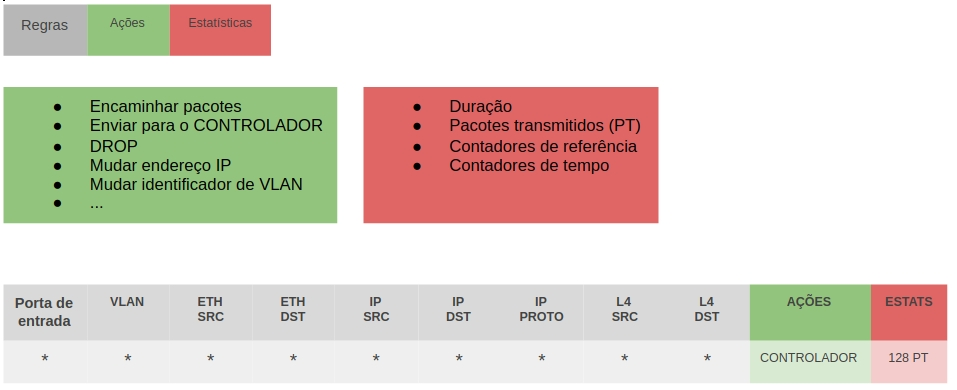
\includegraphics[scale=0.45]{imagens/entrada.jpg}
	\end{center}
	\fonte{Elaborada pelo autor (2021), com base em \cite{guedes:2}}
\end{figure}


As Figuras~\ref{fig:entrada_tabela_fluxo} ilustra as informações da tabela para o encaminhamento de fluxos em SDN. Como a decisão de encaminhamento é feita pelo controlador, então cabe a ele atualizar estas entradas podendo utilizar para encaminhamento tanto partes do cabeçalho que correspondem a camada de rede \textit{L2} ou a camada transporte \textit{L3}, além de poder utilizar a camada \textit{L4} para criação de regras de \textit{firewall} e controle de acesso. Quando um pacote chega no comutador é realizado uma comparação entre cada campo do cabeçalho com seu respectivo campo da tabela entrada. Além das regras utilizadas para verificação, a tabela possui outros dois elementos: ações e estatísticas. De acordo com comparações realizada pelas regras de fluxos, os pacotes são processados conforme as ações de cada regra. As estatísticas são utilizadas para contabilizar os fluxo, tais como quantidade de pacotes, \textit{timeout}\footnote{\textit{Timeout} é um marcador utilizado para determinar quanto tempo essa regra pode durar sem ser utilizada, até se tornar inválida.}, \textit{cookie}\footnote{Cookie é um identificador 64 bits que serve para mapear e armazenar informações relevantes ao controlador sobre determinada regra, muitas regras podem compartilhar do mesmo cookie.} e prioridade \footnote{Prioridade serve para determinar a ordem de precedência que as regras devem ser aplicadas. }. 	



Comutadores comerciais para SDN utilizam circuitos ASIC para realizar processamentos de tarefas específicas como análise de pacotes, \textit{buffering}, escalonamento e encaminhamento de pacotes. No entanto, apesar de avançados, ainda existem desafios para o armazenamento da grande quantidade de fluxos  em tabelas e processamento em picos inesperados de tráfegos. Para resolução de tais problemas, arquiteturas de equipamentos ASIC usam Unidade Central de Processamento (CPU). 
Dessa forma, quando um novo fluxo é adicionado, a CPU verifica a existência de fluxos inativos que estejam sem receber pacotes em um determinado período de tempo pelo campo \textit{timeout}, substituindo essa entrada da tabela pelo novo fluxo, passando ele para ser processado pela ASIC. 
Caso contrário, a própria CPU fica responsável por encaminhar os novos fluxos dessa categoria. Da mesma forma, a Memória de Acesso Randômico Dinâmica (DRAM) pode ser utilizada para armazenamento de \textit{buffer} em caso de picos de tráfegos, para melhorar a eficiência no encaminhamento de pacotes~\cite{nunes-2014}~\cite{gong2015survey}. A CPU pode direcionar fluxos maiores para serem processados pela ASIC enquanto os fluxos menores ficam sendo totalmente processados pela CPU.


\section{Padrão OpenFlow}
\label{sec:openflow}

Dentre os padrões ofertados no mercado para estabelecer uma comunicação entre os comutadores e os controladores, o que mais vem se destacado ao longo dos últimos anos é o \textit{OpenFlow}. Atualmente se encontra na versão 1.5 sendo a versão 1.3 mais amplamente usada em comutadores comerciais, esse padrão vem sendo desenvolvido e mantido pela \emph{Open Network Foundation} (ONF) permitindo que cada vez mais novas possibilidades de aplicações sejam desenvolvidas. O padrão OpenFlow é caracterizado por três componestes: tabelas de fluxos, canal seguro e protocolo OpenFlow.


%Na primeira versão do \textit{OpenFlow 1.0} apenas 12 campos eram permitidos para comparações em cada regra, essa que eram adicionadas em uma única tabela de fluxo armazenada na \ac{TCAM} na qual mais detalhes estão na sessão ~\ref{sub:tabelas}. Sempre que um pacote corresponder a uma regra da tablea o switch aplica as açoes vinculadas a elas, como ilustrados anteriormente na Figura \ref{fig:exemplo_tabel}. A versão atual o \textit{OpenFlow} permite utilizar de 41 campos para criação das regras de \textit{match} podendo ser inseridas em múltiplas tabelas de fluxos. Outra funcionalidade significativa adicionada ao padrão foi o uso de \ac{QoS} já em sua versão 1.3, no qual foi adicionado ações de \textit{queue}. Essa ação permite que sejam criadas filas com diferentes larguras de banda para uma mesma porta física. Sendo assim a ação de \textit{queue} pode adicionar em uma fila com menor ou maior largura de banda permitindo que o fluxo seja melhor balanceado entre diferentes tipos de aplicações. Exemplo, podemos criar uma \textit{queue} de 10\% da largura de banda e uma de 100\% da largura de banda, então especificar que um determinado serviço menos prioritário utilize a ação de enfileirar na \textit{queue} de menor largura de banda, enquanto outros serviços mais prioritários poder utilizar de filas com maior largura de banda.

%Esse padrão fornece três tipos de mensagens para o \ac{NOS}. Primeiro, mensagens de eventos são enviadas para portas destinadas ao controlador quando algum gatilho aciona alguma ação. Segundo, as estatísticas da rede que são geradas e armazenadas em cada dispositivo de encaminhamento são coletadas pelo controlador. E por último, quando um pacote da entrada alcançar o comutador e este não possuir regras na tabela de fluxo para realizar uma operação, o pacote é enviado para o controlador decidir o que deve ocorrer com os pacotes desse novo fluxo. 


%||||||||||||||||||||||||||||||||||||||||||||||||||||||||||||||||||||||||||||||||||||||||||
\subsection{Tabelas de Fluxos}
\label{sub:tabelas}
As tabelas de fluxos são encontradas nos dispositivos de encaminhamento, no qual cada entrada da tabela conta com três principais partes: i) cabeçalho, ii) contadores e iii) ações. Os campos de cabeçalho são utilizados para realizar a verificação do fluxo e assim determinar se estes pertences a determinada regra (\textit{match}). O \textit{OpenFlow} 1.3 conta com 44 campos de cabeçalhos que podem ser utilizados para a formação de um \textit{match}~\cite{nygren2015openflow}. Os campos de contadores armazenam informações para manter o controlador atualizado sobre o status da rede. As ações determinam como o pacote do fluxo será tratado quando um \textit{match} ocorrer. 

\subsubsection{Cabeçalho}
Quando é inserido em um comutador uma entrada na tabela de fluxo que irá gerar um \textit{match} o controlador pode informar um curinga (\textit{ANY}) para os campos que devem corresponder a qualquer valor contido no respectivo campo do pacote. Exemplo, quando o curinga é informado no campo de \textit{MAC\_DST}, significa que qualquer endereço MAC irá corresponder nesse campo. Para ocorrer um \textit{match} o cabeçalho do pacote deve corresponder ao cabeçalho da entrada da tabela de fluxo, exceto os curingas. Caso não haja entradas que formam um \textit{match} com regras específicas, o \textit{OpenFlow} permite que este pacote seja tratado de três formas. Na primeira com a criação de uma regra chamada \textit{table-miss flow}, entrada específica na tabela com prioridade 0 e todos os campos curingas com uma ação de enviar ao controlador. Caso o comutador esteja ligado ao controlador através de outro comutador, é preciso configurar essa regra de modo que a ação da \textit{table-miss flow} envie para a porta vinculada ao segundo comutador intermediário.

\begin{figure}[!htb]
	\caption{\label{fig:pipeline} Exemplo de processamento interno de fluxo em um comutador OpenFlow 1.3}
	\begin{center}
	    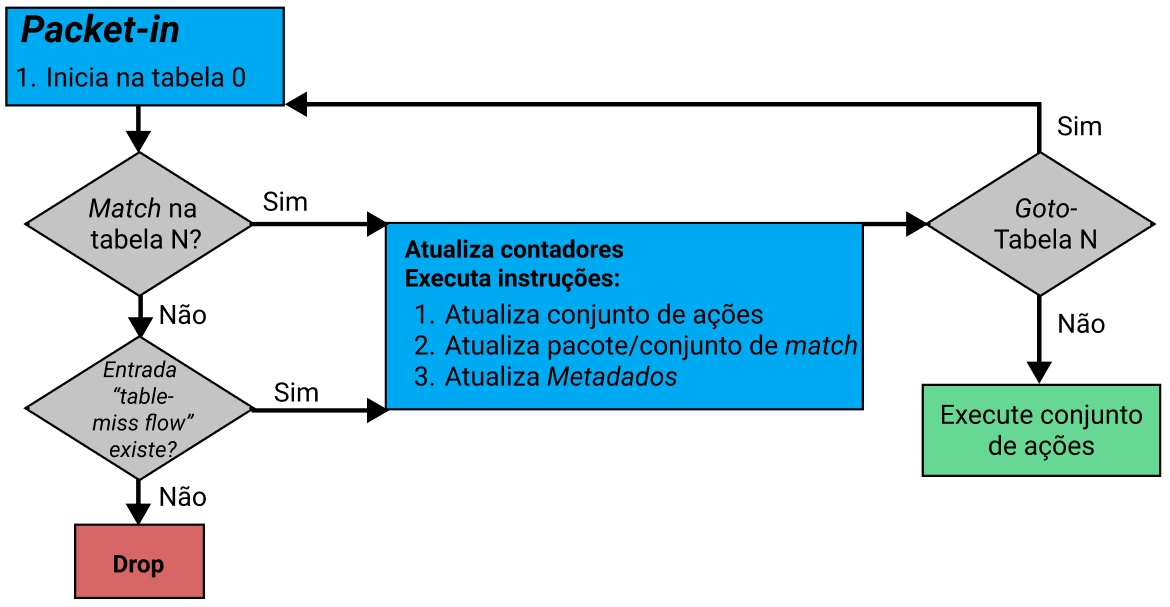
\includegraphics[scale=0.45]{imagens/pipeline.jpg}
	\end{center}
	\fonte{Elaborada pelo autor (2021), com base de \cite{onf2012openflow}}
\end{figure}

 A segunda abordagem é apenas descartar o pacote com a ação \textit{drop}, assim o SDN trabalhará só com fluxos premeditados, e todos os pacotes desconhecidos são descartados. A terceira forma é a utilização de \textit{goto}\footnote{goto é uma instrução utilizada para definir a próxima tabela que deve ser consultada, essa instrução pode apenas avançar o número da tabela.} pulando para análise de regras nas próximas tabelas.


Como ilustra a Figura ~\ref{fig:pipeline}, todos os pacotes que chegam ao comutador passam por uma série de processamento iniciando na tabela 0 com campos do \textit{pipeline} inicializados. Quando ocorre um \textit{match} entre uma das entradas da tabela e o cabeçalho desse pacote é avançado a \textit{pipeline} para a fase de atualização dos contadores dessa regra, aplica o conjunto de instruções e o conjunto de ações. Esse processo pode ocorrer diversas vezes até que as ações de todas as entradas que causaram \textit{match} sejam aplicadas. Caso contenha ações de \textit{output} o comutador pode gerar o pacote de saída definido pelas ações, ou ainda consultar as próximas tabelas de saídas em um novo \textit{pipeline} de processamento. Pacotes enviados pelo controlador podem utilizar somente da \textit{pipeline} que executa instruções, adicionando e removendo entradas ou coletando dados armazenados pelos contadores.


%Como ilustra a Figura ~\ref{fig:pipeline}, todos os fluxos que chegam no comutador iniciam na tabela de entrada 0. Para cada regra correspondente, os contadores relacionados são atualizados e adicionadas as ações correspondentes a um conjunto de ações. Dessa forma, o fluxo é comparado com todas as tabelas existentes e ao terminar as comparações o conjunto de ações é executado. Os campos de contadores são associados a cada regra da tabelas e são utilizados para estatísticas do fluxo. Existem oito tipos de contadores: contadores por tabelas, fluxo, porta, fila, grupo, grupo de \textit{bucket}, \textit{meter} e  \textit{meter band}. A Tabela \ref{tab:contadores} apresenta uma lista com os contadores que todos dispositivos OpenFlow devem conter~\cite{pfaff2012openflow}.

\subsubsection{Contadores}
Os contadores são utilizados para armazenar informações relevantes aos fluxos. A tabela~\ref{tab:contadores} contem os contadores do OpenFlow. Esses são atualizados durante a \textit{pipeline} de processamento dos pacotes e podem fornecer estatísticas de modo que o controlador possa efetuar o melhor gerenciamento da rede, como exemplo, utilizar os contadores de fluxo, \textit{bytes} recebidos e duração para calcular a taxa de transferência relacionada ao fluxo. Assim o controlador pode identificar e reescalonar os fluxos para filas de menor ou maior vazão dependendo de políticas implantadas, ou ainda calcular custo de enlaces dinâmicos pelas estatísticas de portas. Os contadores de duração são obrigatórios e utilizam a precisão dos segundos, estes  são inicializados no momento em que o fluxo é inserido na tabela, e comparados aos campos de \textit{time-out} para determinar que uma regra tenha perdido a validade. Quando a tabela de fluxo esta totalmente utilizada não possuindo mais entradas vazias, os contadores são utilizados para que o próprio comutador decida qual entrada deve ser substituída, evitando assim que esses erros consumam tempo do controlador que possui uma lista de tarefas mais prioritárias em andamento.


\begin{table}[]
\caption{Lista de contadores OpenFlow.}
\label{tab:contadores}
\begin{tabular}{|c|l|l|c|l|}
\cline{1-2} \cline{4-5}
\textbf{Contador} & \textbf{Bits} &  & \textbf{Contador} & \multicolumn{1}{c|}{\textbf{Bits}} \\ \cline{1-2} \cline{4-5} 
Por Tabela de Fluxo &  &  & Por grupo & \multicolumn{1}{c|}{} \\ \cline{1-2} \cline{4-5} 
Entradas ativas & 32 &  & entradas ativas &  \\ \cline{1-2} \cline{4-5} 
Consulta de pacotes & 64 &  & Contador de pacotes &  \\ \cline{1-2} \cline{4-5} 
Pacotes correspondidos & 64 &  & Contador de bytes &  \\ \cline{1-2} \cline{4-5} 
Por entrada de fluxo &  &  & Duração &  \\ \cline{1-2} \cline{4-5} 
Pacotes recebidos & 64 &  & Por métrica & \multicolumn{1}{c|}{} \\ \cline{1-2} \cline{4-5} 
Bytes recebidos & 64 &  & Contagem de fluxo & 32 \\ \cline{1-2} \cline{4-5} 
Duração & 32 &  & Contagem de pacotes input & 64 \\ \cline{1-2} \cline{4-5} 
Por porta &  &  & Contagem de bites de input & 64 \\ \cline{1-2} \cline{4-5} 
Pacotes recebidos & 64 &  & Duração (segundos) &  \\ \cline{1-2} \cline{4-5} 
Pacotes transmitidos & 64 &  & Por métrica de banda & \multicolumn{1}{c|}{} \\ \cline{1-2} \cline{4-5} 
Colisão & 64 &  & Contagem de pacotes & 64 \\ \cline{1-2} \cline{4-5} 
Erros transmitidos & 64 &  & Contagem de bytes & 64 \\ \cline{1-2} \cline{4-5} 
Pacotes recebidos e descartados & 64 &  & Por Fila & \multicolumn{1}{c|}{} \\ \cline{1-2} \cline{4-5} 
Pacotes transmitidos e descartados & 64 &  & Pacotes transmitidos & 64 \\ \cline{1-2} \cline{4-5} 
Erros recebidos & 64 &  & Bytes transmitidos & 64 \\ \cline{1-2} \cline{4-5} 
Duração (segundos) & 32 &  & Duração (segundos) & 32 \\ \cline{1-2} \cline{4-5} 
\end{tabular}
\fonte{Elaborada pelo autor (2021), com base em \cite{onf2012openflow}}
\end{table}

\subsubsection{Instruções}

\begin{table}[!htb]
\caption{Lista de instruções do OpenFlow.}
\label{tab:instruction}
\centering
\begin{tabular}{|l|l|l|}
\hline
\multicolumn{1}{|c|}{\textbf{Instrução}} & \multicolumn{1}{c|}{\textbf{Parâmetro}} & \multicolumn{1}{c|}{\textbf{Descrição}} \\ \hline
Aplica-Ações & Lista de ações & \begin{tabular}[c]{@{}l@{}}Aplica o conjunto de ações vincula-\\ da a entrada imediatamente.\end{tabular} \\ \hline
Limpa Ações &  & \begin{tabular}[c]{@{}l@{}}Limpa o conjunto de ações imedia-\\ tamente.\end{tabular} \\ \hline
Escreva-Ações & Lista de ações & \begin{tabular}[c]{@{}l@{}}Realiza um merge entre a lista de \\ ações atual e a lista de ações pass-\\ ada por parâmetro. Quando uma \\ ação de mesmo tipo ja exista então\\ sobrescreve a ação. Caso não exista, adiciona.\end{tabular} \\ \hline
Escreva-Metadados & \begin{tabular}[c]{@{}l@{}}Metadados/\\ Mask\end{tabular} & \begin{tabular}[c]{@{}l@{}}Insere valor no metadado de acor-\\ do com  os bits da mascára.\end{tabular} \\ \hline
Medidor & \begin{tabular}[c]{@{}l@{}}Limiar de \\ estatísticas\end{tabular} & \begin{tabular}[c]{@{}l@{}}Encaminha o pacote a algum\\ medidor, podendo descartar pacotes \\caso atinja o limiar.\end{tabular} \\ \hline
Goto-Tabela & Id da tabela & \begin{tabular}[c]{@{}l@{}}Indica o id da próxima tabela que\\ deve ser processada durante o pi-\\ peline de processamento.\end{tabular} \\ \hline
\end{tabular}
\fonte{Elaborada pelo autor (2021), com base em \cite{onf2012openflow}}
\end{table}

O conjunto instruções estão vinculados as entradas da tabela de fluxo e servem para realizar alterações em campos do cabeçalho do pacote, alterações no conjunto de ações e alterações da \textit{pipeline} de processamento. O OpenFlow possui seis tipos de instruções que estão listadas na Tabela ~\ref{tab:instruction} em ordem de precedência. É através das instruções que o controlador insere e remove as regras de \textit{match}.
Instruções do tipo \emph{goto} são sempre executadas por último. 

\subsubsection{Ações}
As ações determinam como o dispositivo tratará o fluxo. O conjunto de ações relacionadas a cada entrada da tabela de fluxo é por padrão vazio e são inseridas durante a \textit{pipeline} de processamento das instruções (\emph{e.g.,} Aplica-Ações, Escreva-Ações, \emph{Goto}). Durante o processamento, apenas uma ação de cada tipo pode ser adicionada a lista. Exemplo, quando adicionado ao conjunto de ações uma ação de atualizar a porta \emph{Transmission Control Protocol} (TCP) para outro valor, e outra ação realiza a mesma operação para um valor diferente, esta ação não pode ser inserida a lista de ações, pois apenas uma é permitida. Conforme o processamento vai avançando entre as tabelas com o uso do \emph{goto}, novas ações são inseridas ao conjunto~\cite{nygren2015openflow}. O padrão OpenFlow permite onze tipos de ações, das quais apenas três primeiras são obrigatórias, seis das comumente utilizadas são: 
\begin{itemize}
\item[1] \emph{ Output} é a ação que encaminha o pacote para uma porta específica, como ilustrado na figura \ref{fig:pipeline} quando esta ação é realizada na \textit{pipeline}  com um conjunto de ações, os pacotes são clonados passam pelo mesmo procedimento. Assim cada cópia é enviada por uma porta.
\item[2] Grupo, processa o pacote de acordo com ações determinadas aos seus respectivos identificadores de grupos.
\item[3] \emph{Drop}, ação responsável por descartar o pacote. 
\item[4] Enfileirar, ação que insere o pacote na fila de uma porta configurada conforme políticas de QoS. Uma única porta pode conter diversas filas e cada fila pode ser configurada com sua própria largura de banda. As filas descartam pacotes para manter a largura de banda em seu limite máximo, por exemplo, uma fila configurada para 1~Mb/s descartará pacotes de modo a manter o fluxo em 1~Mb/s. Cada porta pode conter múltiplas filas em diferentes configurações, permitindo o controlador restringir conforme a necessidade.
\item[5] Medidor, direciona o pacote para ser tratado em uma tabela de medidores. Nessa tabela os medidores podem definir limitante de taxas, QoS, largura de banda, entre outros medidores inseridos pelo controlador. Dependendo do resultado desse processamento o pacote pode ser descartado, para se ajustar aos parâmetros do medidor.
\item[6] Copiar campo, ação que pode atualizar os valores de algum campo do pacote. Aplicações de balanceamento de carga de servidores, podem utilizar essa ação para que múltiplos servidores possuam o mesmo endereço IP, distribuindo assim as requisições.
\end{itemize}





%||||||||||||||||||||||||||||||||||||||||||||||||||||||||||||||||||||||||||||||||||||||||||
\subsection{Canal Seguro}
\label{sub:canal}
Também conhecido por canal OpenFlow, este tem o objetivo de conectar cada comutador ao controlador. Por meio deste canal o controlador gerencia as regras das tabelas de fluxos, coleta estatísticas e recebe pacotes \textit{packet-in}. Como uma SDN pode possuir múltiplos dispositivos de encaminhamento, nem sempre é possível criar enlaces diretos entre dispositivos de encaminhamento e controlador, sendo assim, a topologia de rede compartilhada por diferentes usuários também é usada para efetuar o gerenciamento da infraestrutura. Dessa forma toda comunicação realizada entre dispositivos e controlador normalmente são encriptadas utilizando \textit{Secure Socket Layer} (SSL) e \textit{Transport Layer Security} (TLS) para garantir a confidencialidade da comunicação ~\cite{pfaff2012openflow}. 
%||||||||||||||||||||||||||||||||||||||||||||||||||||||||||||||||||||||||||||||||||||||||||
\subsection{Mensagens e Exemplos}
\label{sub:protocolo}
O protocolo OpenFlow é uma das principais partes do padrão. Neste protocolo são utilizados três categorias de mensagens: 
\textit{(i)} \textit{Controlador-Comutador}, são mensagens iniciadas pelo controlador com o objetivo de analisar e gerenciar os estados do comutador. 
\textit{(ii)} Assíncronas, são mensagens geradas pelo comutador para atualizar o controlador sobre informações de eventos de rede que causam mudanças de estados do dispositivo. 
\textit{(iii)} Simétricas, mensagens que podem ser geradas tanto por dispositivo quanto pelo controlador sendo enviadas sem solicitação, utilizadas para inicialização do dispositivo e verificação do canal seguro.  ~\cite{pfaff2012openflow}.


\begin{figure}[!htb]
	\caption{\label{fig:exemplo_tabela} Tabela de fluxo com regras de encaminhamento, \textit{firewall} e comunicação por VLANs.}
	\begin{center}
	    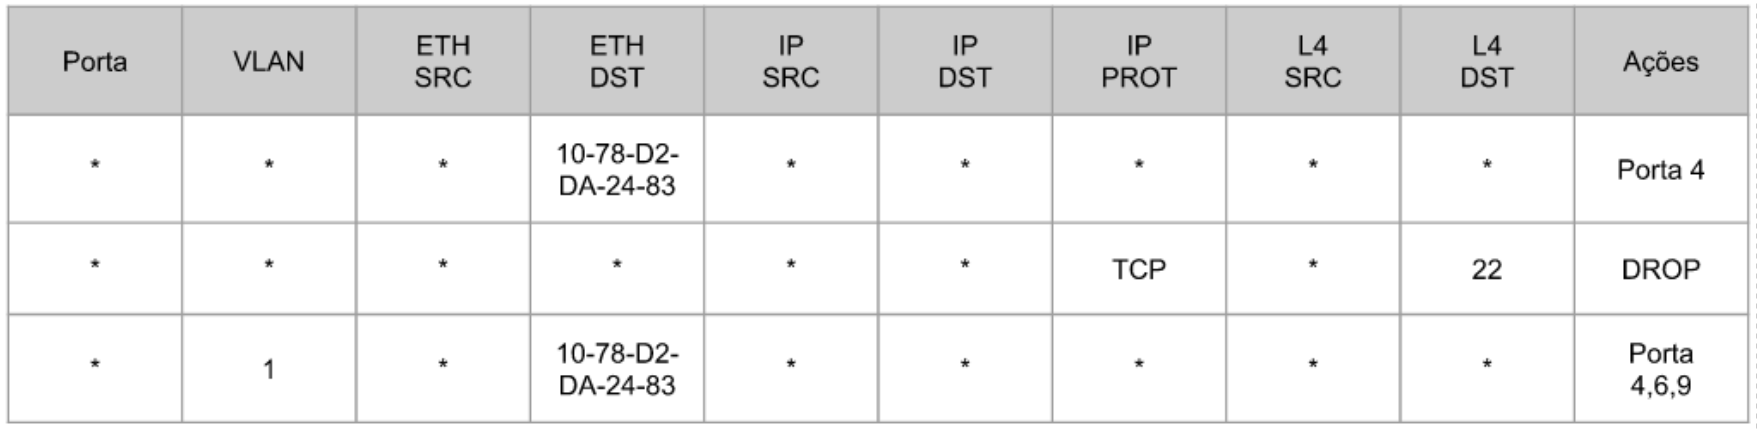
\includegraphics[scale=0.20]{imagens/tabela.png}
	\end{center}
	\fonte{Elaborada pelo autor (2021), com base em \cite{guedes:2}}
\end{figure}

A Figura \ref{fig:exemplo_tabela} contém as principais tuplas que realizam operações sobre o cabeçalho de cada pacote do fluxo, executando assim as ações correspondentes e armazenando estatísticas. O * indica o curinga \textit{don't care}, ou seja, quando o cabeçalho do pacote \textit{OpenFlow} utilizar a entrada da tabela para verificar se são iguais, os campos representados na tabela por \textit{*} resultam em expressão verdadeira para qualquer valor. Segindo essa lógica, a primeira linha da tabela especifica que todos os pacotes que entrarem neste comutador com o endereço de MAC destino igual a \textit{10:78:D2:DA:24:83}, serão encaminhados pela porta física 4. Qualquer pacote que utilizar o protocolo TCP/IP com destino a porta 22 será descartado, ou seja, ele atua como um \textit{firewall} bloqueando qualquer comunicação \emph{Secure Shell Protocol} (SSH). Já a última regra da tabela de fluxo informa que qualquer pacote com a \textit{tag} da VLAN 1 e destino ao endereço físico \textit{10:78:D2:DA:24:83}  terá cópias mandadas para as portas 4, 6 e 9 simultaneamente ~\cite{guedes:2}.

\begin{table}[!htb]
\caption{Principais classes de mensagens suportadas pelo protocolo OpenFlow.}
\centering
\label{tab:mensagens_protocolo}
\begin{tabular}{|l|l|}
\hline
\multicolumn{2}{|c|}{\textbf{MENSAGENS DO PROTOCOLO OPENFLOW}} \\ \hline
\multicolumn{2}{|c|}{\textbf{Controlador para Comutador}} \\ \hline
Características & Solicita as capacidades do dispositivo de encaminhamento. \\ \hline
Configuração & Estabelecer e solicitar parâmetros de configuração do dispositivo. \\ \hline
\textit{Modify-State} & \begin{tabular}[c]{@{}l@{}}Mensagens geradas pelo controlador para efetuar gerenciamento do\\   estado dos comutadores. Dessa forma é possível atualizar inserir e \\ remover tabelas de fluxos no dispositivo\end{tabular} \\ \hline
\textit{Read-State} & \begin{tabular}[c]{@{}l@{}}Mensagem de solicitação de informações dos comutadores, \\ estatísticas, configurações e capacidade.\end{tabular} \\ \hline
\textit{Packet-out} & \begin{tabular}[c]{@{}l@{}}Mensagem \textit{packet-in} devolvida, contendo ações para aplicação imediata \\ do comutador, contém o número da porta de saída. Essa mensagem \\também pode contém as ações de filas e medidores.\end{tabular} \\ \hline
\textit{Role-Request} & \begin{tabular}[c]{@{}l@{}}Mensagem utilizada para configurar ou obter configuração do canal\\ \textit{OpenFlow}, usado em caso de vários controladores, para especificar \\ qual deve ser usado como primário.\end{tabular} \\ \hline
\multicolumn{2}{|c|}{\textbf{Assíncronas}} \\ \hline
\textit{Packet-in} & \begin{tabular}[c]{@{}l@{}}Mensagem enviada quando um fluxo não identificado entra no\\  comutador, pode enviar o pacote completo ou apanas parte de seu \\ cabeçalho, mantendo o pacote armazenado na memória para\\  prosseguir com o encaminhamento de acordo com a resposta do \\ controlador.\end{tabular} \\ \hline
\textit{Flow-Removed} & \begin{tabular}[c]{@{}l@{}}Informam o controlador quando um fluxo é removido da tabela \\ quando seu limite de tempo é excedido ou caso a quantidade \\ pacotes pertencente ao fluxo seja atingida.\end{tabular} \\ \hline
\textit{Port-status} & \begin{tabular}[c]{@{}l@{}}Informa o controlador de mudanças no estado da porta caso ela\\ seja desativada por mensagens de configuração ou por apresentar \\ falhas no enlace.\end{tabular} \\ \hline
\textit{Error} & Informa o controlador quando o comutador apresenta algum erro. \\ \hline
\multicolumn{2}{|c|}{\textbf{Simétricas}} \\ \hline
\textit{Hello} & \begin{tabular}[c]{@{}l@{}}Mensagens enviadas por controladores e comutadores quando a rede \\ é iniciada.\end{tabular} \\ \hline
\textit{Echo} & \begin{tabular}[c]{@{}l@{}}Mensagem do tipo requisição e resposta que podem ser enviadas pelos \\ comutadores ou pelo controlador para verificar problemas em enlaces ou \\ no canal seguro.\end{tabular} \\ \hline
\textit{Experimenter} & \begin{tabular}[c]{@{}l@{}}Mensagem que fornece um padrão para os comutadores \textit{OpenFlow} \\ oferecerem funcionalidades adicionais.\end{tabular} \\ \hline
\end{tabular}
\fonte{Elaborada pelo autor (2021), com base em \cite{onf2012openflow}}
\end{table}

As principais mensagens suportadas pelo protocolo são apresentadas na Tabela ~\ref{tab:mensagens_protocolo}. As mensagens como \textit{Flow-Removed} funcionam da seguinte forma: o controlador adiciona um marcador no momento de criação do \textit{match}, assim indica ao comutador que notifique o controlador quando a regra expirar, seja por tempo ocioso do fluxo, ou por por tempo limite. Essa mensagem é útil para manter o controlador atualizado sobre as configurações dos fluxos sem que haja a necessidade de solicitações de consultas aos comutadores. Já que ao inserir os fluxos ele pode memorizar em caches, e removê-los com esses eventos.

%##########################################################################################
\section{Controlador Floodlight}
\label{sec:floodlight}

O \textit{Floodlight} é um controlador centralizado que utiliza o protocolo \textit{OpenFlow}, possuindo suporte a \textit{multi-threading}, implementado na linguagem \textit{Java}. Ainda oferece através de módulos e aplicações que atuam no gerenciamento da rede.
Dentre as opções de controladores investigadas, \textit{Floodlight} foi identificado como o controlador centralizado com código estável e comunidade de desenvolvimento ativa.
Esses requisitos são essenciais para o desenvolvimento do presente trabalho.
Ainda, \textit{Floodlight} possui total integração com o ambiente de prototipação \textit{Mininet} (detalhado na Seção~\ref{sec:mininet}).

\begin{figure}[!htb]
	\caption{\label{fig:Floodlight-Diagram} Arquitetura modular interna do controlador \textit{Floodlight}.}
	\begin{center}
	    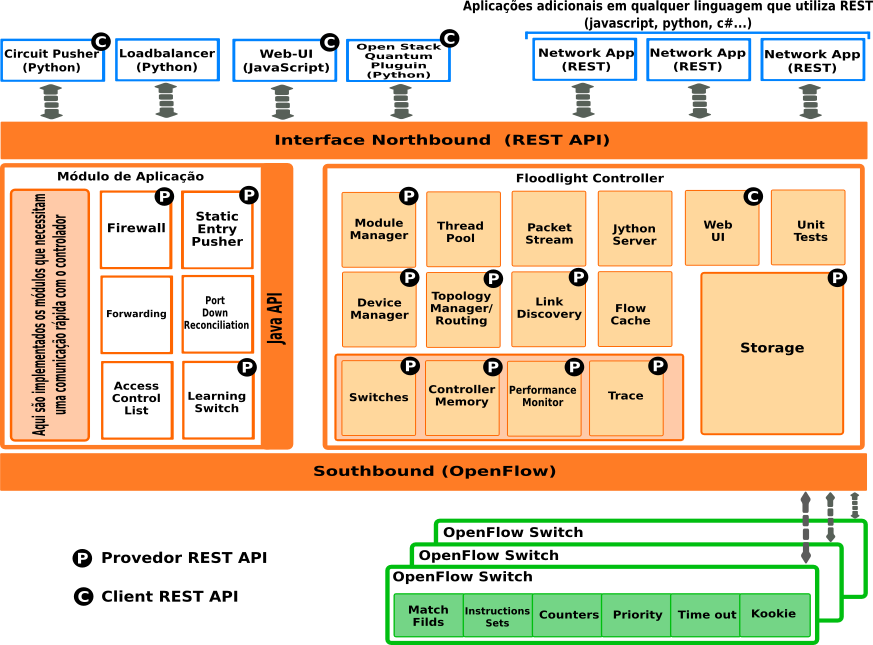
\includegraphics[scale=0.55]{imagens/arquitetura_floodlight_2.png}
	\end{center}
	\fonte{Elaborada pelo autor (2021), com base em \cite{floodlight2012}}
\end{figure}

Sempre que o \textit{Floodlight} é executado, todos os módulos de aplicações também são inicializados, assim as APIs REST expostas pelos módulos ficam acessíveis pela porta 8080, dessa forma todas as aplicações REST seja qual for a linguagem pode recuperar informações e invocar serviços através de URLs.
%||||||||||||||||||||||||||||||||||||||||||||||||||||||||||||||||||||||||||||||||||||||||||
%\subsection{funcionamento}
%\label{sub:funcionamento}

%||||||||||||||||||||||||||||||||||||||||||||||||||||||||||||||||||||||||||||||||||||||||||
\subsection{Aplicações Disponibilizadas}
\label{sub:mecanismo}

A Figura~\ref{fig:Floodlight-Diagram} ilustra a arquitetura atual do Floodlight. Em azul ficam as aplicações independentes de linguagem de programação que fazem requisições REST. Em módulo de Aplicação ficam as aplicações que necessitam comunicações rápidas com o controlador, objetos compartilhados como é o caso da topologia, lista de enlaces, lista de comutadores. Toda informação do controlador é acessível importando as classes de \textit{Floodlight Controller} e implementando as \textit{interfaces}. Os módulos marcados com "\textit{p}", indicam que estes além de poderem ser instanciados por outros módulos podem ser acessados via URLs.
Dentre os módulos e aplicações apresentados pela figura as principais (relacionadas com o presente trabalho) são apresentadas com maiores detalhes nos tópicos:

\begin{itemize}
\item \textit{Firewall}: Aplicação para gerenciar regras de permitir/negar tráfegos específicos ou combinações de regras. Possui um conjunto de APIs REST para adicionar e remover regras de Firewall aplicadas nos comutadores.
\item \textit{Port Down Reconciliation}: Módulo específico para procurar e excluir regras das tabelas de fluxos relacionadas com enlaces que estejam apresentando falhas. Dessa forma o controlador permite reavaliar o caminho e atualizar a topologia de rede, evitando esses enlaces. Este módulo pode gerar problemas em topologias emuladas de grande porte, pois a demora de escalonamento do processador pode gerar \textit{time-out} fazendo com que as regras sejam removidas inesperadamente.
\item \textit{Forwarding}: Este módulo é responsável por tratar as mensagens enviadas pelos comutadores (\textit{e.g.,} \textit{Packet-in}, \textit{Flow-removed}, \textit{Port-status}) e processar as informações das mensagens gerando respostas aos comutadores, como \textit{Add-flow} e \textit{Packet-out}. Este módulo recebe uma \textit{thread} para cada mensagem recebida, entregue conforme o escalonamento de serviços internos do controlador. Por padrão este módulo conduz o encaminhamento proativo e foi utilizado como base na construção das políticas de \textit{Round-Robin}, caminho mais curto reativo e caminho de menor tráfego explicados em detalhes no Capítulo~\ref{cap:algoritimos}. 

\item \textit{Static Flow Entry Pusher}: é uma aplicação para instalar entradas de fluxos nos comutadores manualmente através de URLs. Com um conjunto de APIs REST para inserir remover e atualizar as entradas de cada comutador, permitindo a integração com outras linguagens de programação como o \textit{Python}. A aplicação \textit{Circuit Pusher} ilustrado na Figura~\ref{fig:Floodlight-Diagram} faz o uso desse módulo para gerar caminhos estáticos entre origem e destino.
\end{itemize} 

%||||||||||||||||||||||||||||||||||||||||||||||||||||||||||||||||||||||||||||||||||||||||||
\subsection{Arquitetura do Controlador} 
\label{sub:arquiteturaflood}
Ilustrado na Figura~\ref{fig:Floodlight-Diagram}, o núcleo do \textit{Floodlight} apresenta uma arquitetura modular, para implementar tanto as funcionalidades quanto as aplicações que utilizam a API REST. Entre os existentes módulos do núcleo do controlador estão alguns responsáveis pelo funcionamento e atualização das informações de desempenho e utilização da rede.
Os componentes principais da arquitetura são:

\begin{itemize}
\item \textit{Module Manager}: módulo responsável pela inicialização dos serviços que estão descritos no arquivo de propriedades.
\item \textit{Thread Pool}: é um \textit{wrapper} para \textit{ScheduledExecutorService} que faz o controle de tempo de execução das \textit{threads} de modo periódico ou específico dependendo do serviço.
\item \textit{Packet Streamer}: é um serviço de \textit{streaming} de pacotes que são trocados entre dispositivos de encaminhamento e o controlador.
\item \textit{Floodlight Provider}: possui duas funcionalidades principais, sendo a primeira manusear a conexão entre os comutadores transformando mensagens OpenFlow em eventos que possam ser lidos pelos demais módulos do controlador. A segunda funcionalidade é despachar a mensagem para o módulo responsável pelo tratamento do evento. 
\item \textit{Device Manager}: faz o registro de adição e remoção mantendo atualizados os dados de dispositivos terminais da rede, tal como computadores.
\item \textit{Link Discovery}: módulo responsável por manter o \textit{status} dos enlaces da rede \textit{OpenFlow} atualizados, este módulo dispara pacotes para serem enviados por portas do comutador e assim verificar enlaces ativos e inativos.
\item \textit{Topology Service}: responsável por atualizar as informações da topologia da rede. A topologia pode ser instanciada em qualquer novo módulo para obtenção de informações de comutadores e enlaces, permitindo assim a visão global da infraestrutura.
\item \textit{REST API Server}: este módulo é responsável por expor a API REST através de HTTP. 
\item \textit{Flow Cache}: módulo responsável por tratar eventos de rede, tal como manusear fluxos em caso de falha no enlace.
\end{itemize}

Alguns módulos da arquitetura não são abordados em detalhes, pois não contribuem diretamente para o desenvolvimento de políticas de encaminhamento. 

%##########################################################################################



%\begin{figure}[!htb]
%	\begin{center}
%	    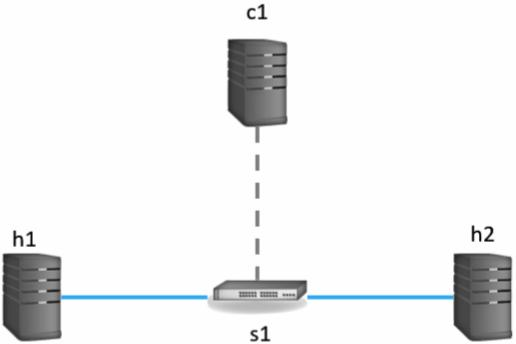
\includegraphics[scale=0.5]{imagens/ping.jpg}
%	\end{center}
%	\caption{\label{fig:ping} Infraestrutura emulada no Mininet para exemplificação de um \textit{ping}. Fonte: desenvolvido pelo autor.}
%\end{figure}

%Alguns comandos tradicionalmente executados em ambientes de experimentação de redes foram adaptados na CLI do Mininet para facilitar o gerenciamento e teste da rede. Por exemplo, quando o  comando\textit{h1 ping h2} é executado, como mostrado na Figura~\ref{fig:ping}, o Mininet interpreta o comando de modo a enviar um pacote ICMP~\cite{mininet}. Assim o Computador h1 envia um pacote ARP para a porta Ethernet, ao receber o pacote o comutador s1 efetuará as operações sobre as tabelas de fluxo, como não existe um fluxo para tratar o pacote o switch s1 gera um \textit{packet-in} mandando a mensagem para o controlador c1. Ao receber a mensagem o controlador o tratará como um um \textit{broadcast} gerando um evento \textit{packet-out} que realizará o \textit{flood} em todas as portas do comutador s1. Quando a mensagem chegar ao Computador h2, ele realiza a resposta, que ao ser processada novamente pelo controlador fará a inserção de do fluxo na tabela do comutador s1.

%##########################################################################################
\section{Considerações Parciais} 
\label{sec:consider}

Este capítulo faz uma revisão de literatura sobre SDN, detalhando seus principais componentes arquiteturais, focando na definição de fluxos e atuação dos controladores.
Em um segundo momento, uma revisão foi apresentada sobre o protocolo \textit{OpenFlow}, um padrão aberto para configuração dos dispositivos em SDN.
\textit{OpenFlow} oferece ao controlador três principais funcionalidades, sendo elas: mensagens de eventos, estatísticas da rede, e requisições de \textit{packet-in} utilizadas quando houver falta na entrada das tabelas de fluxos dos dispositivos de encaminhamento.

Dentre os diversos controladores apresentados está o Floodlight, escrito na linguagem de programação \textit{Java} utiliza o protocolo \textit{OpenFlow} para configuração dos dispositivos de encaminhamento. Por ser o controlador alvo do presente trabalho, a arquitetura do Floodlight foi discutida em detalhes.

O próximo Capítulo~\ref{cap:algoritimos} apresenta os quatro principais algoritmos aplicados para realizar o encaminhamento dos fluxos em SDN. Dois deles utilizam o caminho mais curto, um de abordagem reativa e outro proativa, em que visam o caminho de menor quantidade de saltos. Os outros dois algoritmos fazem o uso de múltiplos caminhos de acordo com estratégias próprias para seleção de rotas alternativas e balanceamento do tráfego. 
